\chapter{Biological Background}\label{chap_background}

In this chapter we will explore the nature of structural variations, discuss the mechanisms that may be behind their formation, and their effect on phenotypes and disease. We will then describe high-throughput sequencing and discuss the typical informatics pipelines that researchers create to analyze sequencing data, placing SV detection within the context of the other types of computation that must be done to support end-to-end analysis. Finally, we will discus the challenges that the increasing number and size of sequencing data sets represent.

\section{Structural Variations}

As we described in the introduction, structural variations (SVs) are rearrangements, relative to some reference genome sequence, of sequences of DNA with a length longer than 40 or 50bp. These can take the form of deletions of reference sequence, insertions of novel sequence, duplications of sequence, inversions of orientation of a stretch of sequence with respect to the rest of its chromosome, or translocations of sequence from one chromosome to another. Deletions, insertions, and duplications are also frequently referred to as \emph{copy number variations} (CNVs). In addition, many complex SVs exist in which these simple SV types are combined.

SVs can occur and become part of a gene pool on several different biological and time scales. On the smallest level, SVs can rearrange the genomes of individual cells within an organism. If the SV contributes to the cell's ability to proliferate, or occurs in conjunction with another mutation that does so, it can give rise to a tumor, or a new subpopulation or clone within an existing tumor. On a population scale, the genomes of individuals within a species harbor SVs with respect to one another, either because they were transmitted through the germline or because they arose \emph{de novo} in certain individuals. Finally, on a larger scale, SVs within a species may become fixed, contributing to differences between the genomes of varying species on an evolutionary scale.

\subsection{SV Effects on Phenotype and Disease}

On all of these levels, SVs are associated with differences in phenotypes and have been shown to associate with many types of disease, making them an important area of study. Of course, our knowledge of these effects has been shaped by the types of SVs that researchers have been able to detect in the past several decades given the assays at their disposal and the scale at which samples could be analyzed. These limitations have biased our understanding towards the large variants with large effect sizes that were discoverable before the advent of modern array and sequencing technologies. 

Cancer genomes contain many SVs that have been linked to tumor progression. The famous Brc-Abl mutation~\cite{Kurzrock:2003bz} mentioned previously is the most famous example of a fusion gene, in which portions of the genome coding for two different genes are made adjacent due to an SV. This results in the creation of new gene which can take on novel functions, which in turn drive cancer growth. Fusion genes can be caused through any type of SV that causes a novel adjacency between regions of the genome, including deletions, duplications, translocations, and inversions, and there have been dozens of recurring fusion genes identified across varying cancers to this point~\cite{Annala:2013ks}. In another example, the genomic locus that contains the \emph{MYC} gene, which among other functions regulates cell proliferation~\cite{Eilers:2008jk}, is frequently duplicated multiple times in breast cancer cells~\cite{Escot:1986tn}. These duplications change the amount of protein made by the cell, causing a dosage-related defect in cell regulation. In other cancer cells, a dramatic process called \emph{chromothripsis} has been observed, in which entire chromosomes appear to ``shatter'' and then be pieced back together. This gives rise to hundreds of SVs, some of which can promote cancer development~\cite{Stephens:2011bm}. On the other end of the spectrum in terms of variant size, small deletions of less than 150bp in untranslated coding regions of genes have been observed to contribute to aberrant gene expression in leukemia~\cite{Hosokawa:1998wi}.

On the scale of the human population, SVs and CNVs have been implicated in a variety of diseases (for a comprehensive recent review see Weischenfeldt et al.~\cite{Weischenfeldt:2013fm}). The best studied of these are large CNVs, including deletions or duplications of genes. These can can include variants that arise \emph{de novo} in individuals, either giving rise to rare disorders~\cite{Lupski:1998ip} or contributing to the risk of more common conditions such as Crohn's disease~\cite{McCarroll:2008jt}, autism~\cite{Sebat:2007bs}, and schizophrenia~\cite{Walsh:2008kp}. However, most CNVs in the human genome are polymorphic within the population and contribute to human genetic diversity~\cite{McCarroll:2008p265}. The rise of microarrays and high-throughput sequencing has sped the discovery of smaller variants that affect coding sequence by deleting exons. To give one recent example, an 8kb deletion of an exon in the BAG3 gene has been tied to risk for cardiomyopathy~\cite{Norton:2011ev}. \todo{etc.}

There are also numerous examples of deletions that affect human phenotypes even though they do not directly overlap with the coding regions of genes, instead interacting with regulatory elements that control gene expression levels. For example, deletions ranging from 36kb to 319kb in size that are over one megabase away from the SOX9 gene locus can alter its expression by removing an enhancer element, giving rise to a rare cleft palate syndrome called Pierre Robin sequence~\cite{Benko:2009dq}. Expanding on this idea, a survey of CNVs between inbred mouse strains showed that 28\% of gene expression differences between strains could be statistically explained by CNVs, but that only 7\% of the identified CNVs directly overlapped one of the differentially expressed genes, suggesting that SVs may shape many aspects of organism phenotypes in complex ways~\cite{Cahan:2009ef}. In another dramatic example from other species, the well-studied stickleback fish, which has repeatedly evolved adaptations to fresh water in several locations around the world as it moved from the sea into lakes, owes one of those adaptations, the loss of spines on its pelvis, to recurrent sub-2kb deletions of an enhancer that regulates the Pitx1 gene~\cite{Chan:2010hz}.

\todo{This last case points to the value that can be gained by studying SVs that have been shaped by, or helped to shape, evolutionary processes. Hahn gene duplications.. Ventura segmental duplications in gorilla.. Gibbon karyotype.. }

\subsection{Mechanisms and Signatures of SV Formation}\label{section_sv_mechanisms}

Given that many of the phenotypic effects of SVs described above are deleterious to the organism, it is natural to ask how they arise in genomes. Biologists have identified several different mechanisms that can cause SVs. By studying many of the genomic disorders mentioned in the previous section, geneticists found that often CNVs recur in different individuals at the same locations in the genome. Examining these locations revealed that they are homologous to sequences repeated elsewhere in the genome in the form of segmental duplications, stretches of DNA that are over 1kb in length with greater than 90\% sequence identity~\cite{Sharp:2006fy}. This helped to identify the process of non-allelic homologous recombination (NAHR)~\cite{Liu:2012if}. In the best studied form of NAHR, the cell attempts to repair DNA in the cell that has suffered double-stranded breaks (DSBs). To do so, it attempts to find homologous DNA in the nucleus that can be used as a template to repair the broken strand. However, repeats in the genome provide the opportunity for DNA from the wrong genomic location to be used in this repair process, creating genomic breakpoints in the repaired DNA. In mammals, as little as 295bp of non-allelic homologous sequence can be responsible for NAHR events~\cite{Liskay:1987wt}. The human genome contains many copies of transposable elements, including 500,000 of the LINE family and over one million of the \emph{Alu} family, with average lengths of 6kb and 300bp, respectively. Both \emph{Alu}~\cite{Lehrman:1985tn} and LINE~\cite{Robberecht:2013kw} are frequently involved in NAHR events. As these and other transposons copy themselves into new locations in the genome, they also give rise to their own class of SV, mobile element insertions (MEIs), which leave their own signatures of small tandem site duplications (TSDs) at either end of the insertions.

In contrast to NAHR, other mechanisms can create SVs without extensive sequence similarity at the breakpoint. Non-homologous end joining (NHEJ) and microhomology mediated end joining (MMEJ) are two such processes~\cite{Hastings:2009fv}. Both of these mechanisms involve the repair of DSBs in the cell and typically result in SV breakpoints that have very small (less than 20bp) homologies on either side. Other processes of SV formation that leave a signature of microhomologies at the breakpoint are Fork Stalling and Template Switching (FoSTeS)~\cite{Lee:2007fy} and microhomology-mediated break-induced replication (MMBIR)~\cite{Hastings:2009fv}. In these models, as the cell replicates all of its DNA two replication forks can switch DNA templates, causing complex structural variations to form. Finally, the chromothripsis process mentioned above also gives rise to microhomologies~\cite{Liu:2011p1751}.

Given that different SV formation mechanisms have different signatures that can be determined by the presence of varying amounts of duplication or homology at or near the breakpoints, it is possible to analyze SVs to gain insight into their formation in different contexts. For example, Conrad et al.~\cite{Conrad:2010if} surveyed CNVs from 40 unrelated individuals using a targeted sequencing method that enabled them to determine exact sequences around the breakpoints of some events. They found that although the best studied human genomic disorders are due to recurrent SVs caused by NAHR, NHEJ and MMEJ were responsible for the great majority of CNVs they were able to detect, a result later confirmed by the 1000 Genomes Project~\cite{Mills:2011p1611}, although studies in mice have found that MEI may be more frequent albeit harder to detect~\cite{Yalcin:2011tm}. \todo{cancer?} In Chapter~\ref{chap_breakpoint_analysis}, we will discuss efforts to analyze the sequence context of genomic rearrangements between species.

\section{High-Throughput Short-Read Sequencing}\label{section_sequencing}

The pace of analysis of genome rearrangements and SVs has risen dramatically with the widespread adoption of high-throughput short-read sequencing (for a review see Shendure and Ji~\cite{Shendure:2008jh}). In early projects to interrogate SVs in DNA samples researchers had to painstakingly map individual variants using time-consuming microscopy (for very large rearrangements), fluorescence in situ hybridization (FISH), southern blotting, or polymerase chain reaction (PCR) assays~\cite{Aten:2008dh}. The development of microarray technology allowed simultaneous testing of many genomic probes on a sample, although the probes had to be developed using prior knowledge of what variants to expect. Short-read sequencing, however, allows direct DNA sequence data to be collected in a relatively unbiased way from the entire genome, overcoming these limitations.

High-throughput short-read sequencing technology is currently dominated by Illumina, Inc. (San Diego, CA), and unless otherwise noted we will be referring to data generated by Illumina instruments when we refer to short-read or next-generation sequencing data in this document. The Illumina sequencing process begins with creation of genomic DNA library, which has billions of small fragments of DNA, sheared randomly across the genome, with adapter sequences attached to the ends. These adapters attach randomly to locations on the surface of the sequencing instrument's \emph{flow cell}, and then are amplified in place to form clusters on the flow cell, each consisting of thousands of copies of a DNA fragment from the library. The sequencer then initiates a process in which the complements of each strand of DNA in the clusters are synthesized one base at a time. Each complementary base added to the new molecule contains a fluorescent tag, and the instrument takes a picture of the flow cell at each step. Pooling the color signal from each strand in a cluster, the sequencer optically analyzes the image from each time step to call the base at that position in each cluster. Because all clusters can be analyzed simultaneously in a single flow cell image, Illumina's sequencing instruments can now process billions of fragments at the same time. Illumina's HiSeq 2500 instrument, the current throughput leader, can produce 1.2 billion paired-end reads, or 120Gb of data, in 27 hours. 

While this technique produces unprecedented amounts of sequencing data, the downside is that read lengths are limited by the extent to which the synthesis process can be regulated and kept in sync across all of the clusters on the flow cell. In Illumina's current high-throughput instruments, this limits read lengths to 100bp or 150bp. The downsides of this can be mitigated somewhat through techniques that sequence both ends of a DNA fragments, producing the paired-end reads referred to earlier. If the size of the fragment is approximately known, the distance between the two sequenced ends can be estimated, as we will discuss in detail in Section~\ref{section_read_pair}. These paired-end techniques typically use fragments of between 250 and 500bp, although in some cases \emph{mate pair} fragment sequencing can produce reads from the ends of much larger fragments (6-8kb).

Because nearly half of the human genome is made up of repetitive elements, the analysis of the short reads produced by these sequencing technologies present a unique set of challenges~\cite{Treangen:2011p1810}. As we mentioned earlier, repetitive elements such as \emph{Alu} and LINE appear many times in the genome. If a read, or pair of reads, falls entirely within a single repetitive element, it will be impossible to determine the location in the genome it came from if there has not been enough sequence divergence of the repeat over evolutionary time to distinguish it from the others. Because many SV formation mechanisms depend on sequence homologies at the breakpoints, they are particularly likely to fall into repeats in the genome, complicating the task of SV detection from short-read data.

In addition to making SV detection difficult, short-read sequencing -- by the unprecedented volume of data it produces -- also presents challenges to developing scalable infrastructure and algorithms for processing sequencing data in general. We will return to the problem of SV detection in the next chapter, and in the remainder of this chapter will give an overview of the applications of high-throughput sequencing data, and will discuss the computational challenges they represent.

\subsection{Sequencing Analysis Pipelines}\label{section_pipelines}

To transform raw sequencing reads into usable information typically requires a series of discrete steps. As genomic bioinformatics has matured, these have been increasingly modularized and made into components that can be connected together to create analytics pipelines designed for particular applications. In this section, we will describe pipelines for several of the most popular applications of high-throughput sequencing.

\subsubsection{DNA Resequencing}

As we mentioned in Chapter~\ref{chap_introduction}, resequencing projects attempt to identify variants present in the genomic DNA of samples from a population for which there exists a reference sequence. Variants can then be specified in standard formats (typically VCF, the Variant Call Format~\cite{Danecek:2011gz}) that describes them in terms of the sequence and coordinates of the reference. These can then be used in study designs such as case/control or genome wide association studies (GWAS), or, in clinical contexts, can be searched directly using prior knowledge for variants likely to be associated with diseases or conditions.

\begin{figure}
\centering
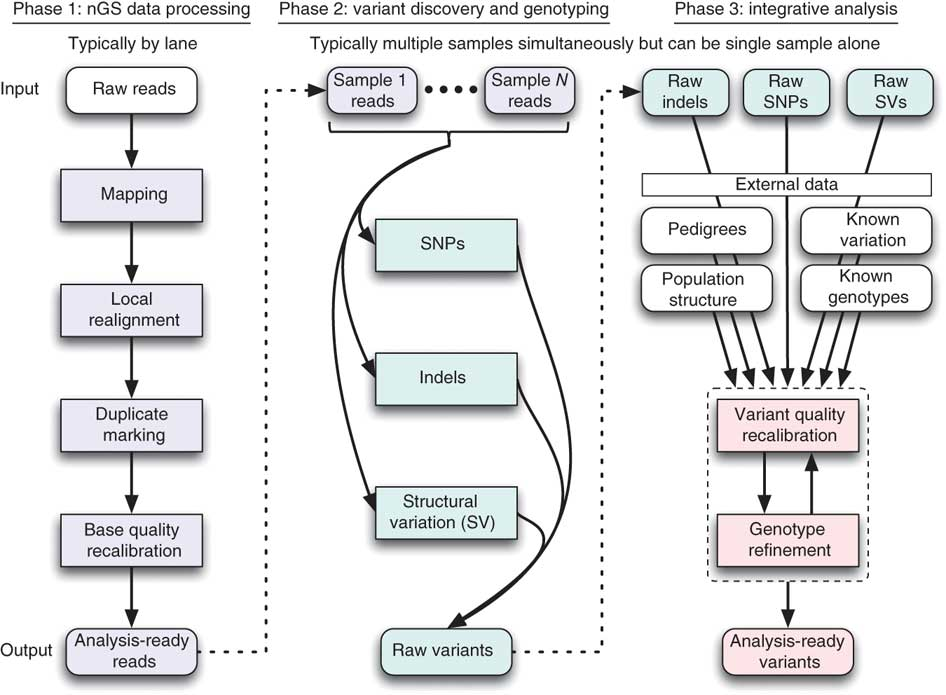
\includegraphics[width=1\textwidth]{figures/ng-806-F1.jpg}
\caption[An example of a computational pipeline for high-throughput short-read DNA resequencing projects.]{An example of a full computational pipeline for high-throughput short-read DNA resequencing projects. This figure describes the Genome Analysis Toolkit (GATK) best practices pipeline, and is representative of the computational steps involved in a full resequencing pipeline designed to process many samples simultaneously. Reprinted by permission from Macmillan Publishers Ltd: Nature Genetics 43:5pp491-498~\cite{DePristo:2011fo}, copyright 2011}
\label{gatk_pipeline}
\end{figure}

Figure~\ref{gatk_pipeline} shows a high-level representation of the steps involved in a large-scale resequencing project using the Genome Analysis Toolkit~\cite{DePristo:2011fo}. The main components are:

\begin{enumerate}
\item \textbf{Quality Control and Data Preparation.} Although not shown in Figure~\ref{gatk_pipeline}, most pipelines typically begin by running a set of reports to assess the quality of the raw data, often with a standardized QC suite such as FastQC~\cite{fastqc} and data preparation steps that include trimming the portions of the input sequences that have base calls with low confidence scores or that contain sequence that matches known artifacts of the sequencing process (adapter trimming). These components operate on raw data in the FASTQ format~\cite{Cock:2010ky}.

\item \textbf{Read Mapping.} In this phase, reads are mapped to the reference genome to find their most likely coordinates of origin. There exist a wide variety of short-read mappers that are heavily optimized for the task of aligning short DNA sequences to reference genomes (for a survey from several years ago see Li and Homer~\cite{Li:2010p10}). These typically use some form of a seed-and-extend strategy, in which exact matches of portions of the input read to the reference genome are found quickly using pre-computed indices. These indices can take the form of hash tables or some form of enhanced suffix array, or more popularly, the suffix trie equivalent FM-index~\cite{Ferragina:2000vl}, which uses the Burrows-Wheeler Transform (BWT)~\cite{Lossless94ablock-sorting} to convert a suffix trie into a highly compressed structure that is particularly useful for indexing highly repetitive genome sequences while still giving fast (under most conditions linear in the length of the query pattern) lookup times. These exact matches are then extended using direct comparisons or through dynamic programming techniques such as the Smith-Waterman alignment algorithm~\cite{Smith:1981up}. Examples of hash-based aligners include Novoalign~\cite{novoalign} and MOSAIK~\cite{2013arXiv1309.1149L}, while BWA~\cite{Li:2009p836} and Bowtie 2~\cite{Langmead:2012jh} are popular BWT-based aligners. The output of this step is typically in the Sequence Alignment/Map (SAM) format~\cite{Li:2009vz}, which in addition to the reads stores their alignment coordinates on the reference genome, mapping quality scores, and information about mismatches to the reference.

\item \textbf{Local Realignment, Duplicate Marking, and Recalibration.} In some pipelines there is often an additional quality control step after read mapping. PCR amplification in the preparation of sequencing libraries from DNA samples can give rise to duplicate fragments, which are typically identified and removed at this point. In addition, this step can include a more expensive realignment phase for groups of reads that appear to span short insertions and deletions (indels, typically under 40bp in size), and a recalibration of the base call quality scores reported by the sequencer based on the empirically observed distribution of mismatches between the reads and the reference sequence~\cite{DePristo:2011fo}.

\item \textbf{Variant Calling.} The next phase includes calling of single nucleotide variants (SNVs), indels, and SVs. To call SNVs and indels, algorithms examine each possible variant indicated by mismatches of reads to the reference. They typically evaluate the number of reads supporting the variant against the total number of reads at that location, as well as prior beliefs, in a Bayesian framework. Popular SNP and INDEL callers include the GATK~\cite{McKenna:2010p1051}, SAMtools~\cite{Li:2009vz}, and SOAPsnp~\cite{Li:2009p1236}. In some cases, multiple samples from a population are examined simultaneously, giving additional power to detect variants in that population. We will discuss SV callers in more detail in Chapter~\ref{chap_related_work}.

\item \textbf{Integrative Analysis/Filtering.} After raw variants have been called, additional sources of outside information can be used to adjust their confidence scores or filter out false positives. This can include data from existing catalogs of genomic variants or knowledge about the population structure of the samples. If multiple samples from the same pedigree are being sequenced, data can be reconciled based on the principles of inheritance. DePristo et al.~\cite{DePristo:2011fo} describe one such set of filters appropriate for a large scale study involving many individuals from a population. In Section~\ref{section_aml_pipeline} we will describe a simple filtering scheme we implemented for a cancer sequencing project.

\end{enumerate}

\subsubsection{Other Sequencing Applications}

In addition to DNA resequencing to detect genomic variants, there are many other applications of short-read sequencing. We will not go into detail on how each works, but will briefly list the goals and major informatic components of several of the most common so that we can address a full picture of the computational scaling challenges that short-read sequencing represents. 

\begin{itemize}
\item \textbf{RNA-seq.} In RNA-seq (see Oshlack et al.~\cite{Oshlack:2010kr} for a review), the goal is to interrogate the expression of genes across samples, for example in different disease conditions. Rather than sequencing DNA, libraries are constructed from RNA taken from the sample. Similarly to DNA resequencing, the reads are QC'd and aligned to the reference genome, although there are read mappers especially designed for RNA-seq that include functionality to map reads over exon junctions. The reads that map to annotated genes on the reference are then analyzed and quantified to determine  the genes that are being expressed in the sample, along with their relative expression levels and isoforms.

\item \textbf{ChIP-seq} The intent of ChIP-seq (reviewed by Park~\cite{Park:2009gl}) is to determine the locations in which DNA, or the chromatin that contains it, is being bound by protein transcription factors or modified, with the ultimate goal of determining the modifications that are driving gene expression. In this case fragments of DNA that are bound to the protein of interest are preferentially separated and sequenced. After read trimming and mapping, the locations of binding events can be identified by searching for ``peaks'' of coverage on the reference genome.

\item \textbf{\emph{de novo} Assembly} When there is no reference genome present for the organism being sequenced, the goal is to try to reconstruct the full sequence of the input genome based only on the short reads. A full discussion of \emph{de novo} assembly algorithms is beyond the scope of this section; for a review see Nagarajan and Pop~\cite{Nagarajan:2013cq}. The general approach is to build a graph representing overlaps between the reads in the form of either a string graph~\cite{Myers:2005iq} or a \emph{de Bruijn} graph, and then walk the graph to determine the underlying sequence. This is complicated by the fact that mammalian genomes are highly repetitive. The need to construct a graph data structure linking all of the input reads means that assembly is typically an extremely memory-intensive process, making it difficult to distribute computation.

\end{itemize}

There are of course additional sequencing applications, including workflows specifically designed for cancer-related projects and metagenomics, which aims to discover all of the microorganisms present in a diverse sample. 

\subsection{Big Data from Sequencing}\label{section_seq_big_data}

All of these sequencing applications are creating an enormous amount of data that is pushing the limits of the computational infrastructure and algorithms used by biologists. For example, the European Bioinformatics Institute currently stores multiple petabytes of genomic data, and that amount has been taking less than one year to double since the advent of high-throughput sequencing in 2008~\cite{Marx:2013dz}. This has led to increasing calls for new bioinformatics strategies for storing, managing, sharing, and processing that data. An early recognition of the fact that computational requirements would soon outstrip the capacity of the prevailing model of processing data on local servers in individual laboratories created a movement towards centralized databases and processing on remote servers enabled by standardized data formats and annotations~\cite{Stein:2008gh}. After the creation of large scale cloud compute services, bioinformatics leaders quickly realized their potential to ease the burden of processing sequencing data~\cite{Stein:2010gp,Schatz:2010js,Schadt:2010dp}. In particular, they noted that cloud computing would allow the scaling of compute infrastructure to meet demand, rather than having to plan for, acquire, and maintain compute clusters capable of handling the predicted peak load. In addition, cloud computing offers a potential solution to the problem of sharing large data sets in the highly collaborative field of genomics; by storing large data sets in the cloud that are accessible to multiple groups, collaborators could become less dependent on the prevalent strategy of sharing data by shipping hard drives to one another. Several of these arguments also noted that cloud computing is a natural fit for creating distributed algorithms that can be scaled to larger data sets by adding more compute resources, in particular through the use of the MapReduce programming model~\cite{Schatz:2010js,Schadt:2010dp}. We will return to the topic of cloud computing in Chapter~\ref{chap_framework}, where we will develop a framework for detecting SVs in MapReduce. Before we do so, however, we will review existing algorithms for SV detection in Chapter~\ref{chap_related_work}.
